
As a starting example, we consider a compartment pharmacokinetic model for a single patient.
The patient receives multiple doses at regular time intervals and the drug plasma concentration is recorded over time.
Our goal is to infer the physiological parameters of the patient, pertinent to the drug's pharmacokinetics, and the measurement error.

\subsection{Pharmacokinetic model and clinical event schedule} 

The two compartment pharmacokinetic model describes how the drug circulates in the patient's body, until it is cleared out (Figure~\ref{fig:twocpt}).
The drug is orally administered and therefore enters the system through the gut.
Once the drug is introduced in the system, the \textit{natural evolution} of the system is described by a system of ODEs.
In the case of a two compartment model with a first-order absorption from the gut, the system is the following:
%
\begin{eqnarray*}
  \frac{\mathrm d y_\mathrm{gut}}{\mathrm d t} & = & - k_a y_\mathrm{gut} \\ 
  \frac{\mathrm d y_\mathrm{central}}{\mathrm d t} & = & k_a y_\mathrm{gut} - \left (\frac{CL}{V_\mathrm{cent}} + \frac{Q}{V_\mathrm{cent}} \right) y_\mathrm{cent} + \frac{Q}{V_\mathrm{peri}} y_\mathrm{peri} \\
  \frac{\mathrm d y_\mathrm{peri}}{\mathrm d t} & = & \frac{Q}{V_\mathrm{cent}} y_\mathrm{cent} - \frac{Q}{V_\mathrm{peri}} y_\mathrm{peri}
\end{eqnarray*}
%
with
\begin{itemize}
  \setlength\itemsep{0em}
  \item $y(t)$: the drug mass in each compartment (mg)
  \item $k_a$: the rate constant which the drug flows from the gut to the central compartment (h$^{-1}$)
  \item $Q$: the clearance at which the drug flows back and forth between the central and the peripheral compartment (L/h)
  \item $CL$: the clearance at which the drug is cleared from the central compartment (L / h)
  \item $V_\mathrm{cent}$: the volume of the central compartment (L)
  \item $V_\mathrm{peri}$: the volume of the peripheral compartment (L)
\end{itemize}

\begin{figure}
  \begin{center}
  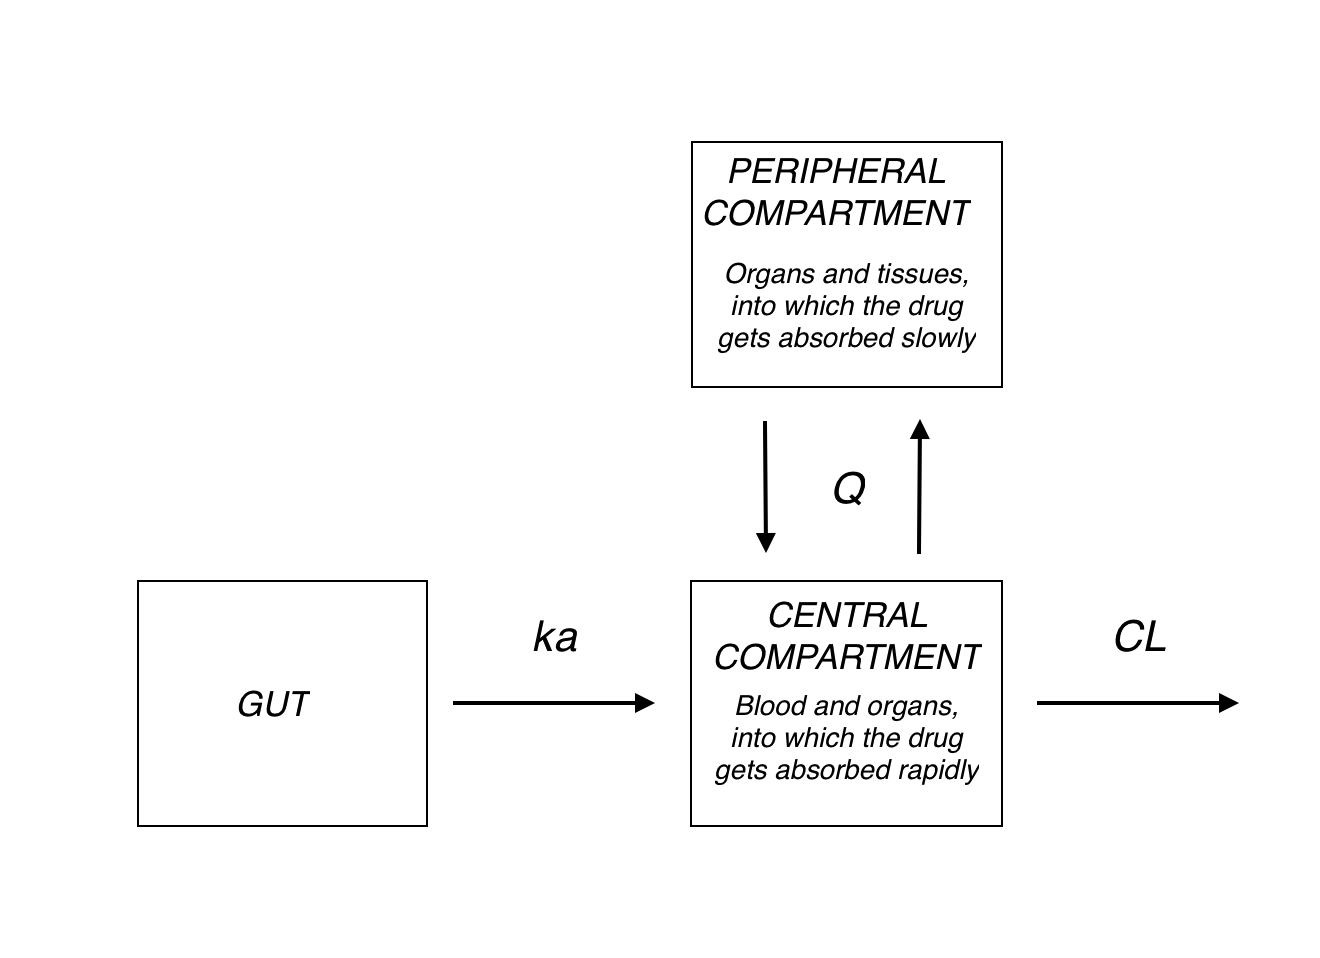
\includegraphics[width=5in]{../figures/TwoCptNice.png}
  \caption{Two compartment model with first-order absorption from the gut.}
  \label{fig:twocpt}
  \end{center}
\end{figure}

During the trial, the patient receives a dose of 1,200 mg every 12 hours, until they have received a total of 14 doses.
Measurements are taken shortly after the first, second, and last doses, and at regular intervals during the treatment.
Both intervention and measurement events are described by the event schedule, which follows the convention established by NONMEM.
This means the user must provide for each event the following variables: \texttt{cmt}, \texttt{evid}, \texttt{addl}, \texttt{ss}, \texttt{amt}, \texttt{time}, \texttt{rate}, and \texttt{ii}.
Appendix~\ref{app:event} reviews the role of each variable.

\subsection{Statistical model}

We define a generative model.
Given a treatment, $x$, and the physiological parameters, $\{ k_a, Q, CL, V_\mathrm{cent}, V_\mathrm{peri} \}$, we obtain the exact drug plasma concentration, $c$, by solving the relevant ODE.
Our measurements, $y$, are a perturbation of $c$ because of our measurement error.
We model this error using a lognormal error, that is
\begin{equation*}
  \log y \sim \mathrm{Normal}(\log c, \sigma^2),
\end{equation*}
where $\sigma$ is a standard deviation we wish to estimate.
The deterministic computation of $c$ along with the measurement model, defines our likelihood function $p(y \mid \theta, x)$, where $\theta = \{ k_a, Q, CL, V_\mathrm{cent}, V_\mathrm{peri}, \sigma \}$.

It remains to define a prior distribution, $p(\theta)$.
Our prior should allocate probability mass to every plausible parameter value and exclude patently absurd values, e.g. the volume of the central compartment is on the order of one liter, but it cannot be the size of the Sun.
In this simulated example, our priors for the individual parameters are based on population estimates from previous (hypothetical) studies.
Suggestions for building priors can be found in references \cite{Gabry:2017, Betancourt:2020, author:0000}.

\subsection{Specifying a model in Stan}

We can now specify our statistical model using a Stan file.
From R, we then run inference algorithms which take this Stan file as an input.

To define a model, we need a procedure which returns the log joint distribution, $\log p(\mathcal D, \theta)$.
Our first task is to declare the data, $\mathcal D$, and the parameters, $\theta$, using the coding blocks \texttt{data} and \texttt{parameters}.
It is important to distinguish the two.
The data is fixed.
By contrast, the parameter values change as HMC explores the parameter space, and gradients of the joint density are computed with respected to $\theta$, but not $\mathcal D$.

\begin{lstlisting}[style=stan, numbers=none] 
  data {
    int<lower = 1> nEvent; 
  }
 
\end{lstlisting}
